\section{Language Models}

A language model takes a sequence of word vectors and outputs a sequence of predicted word vectors by learning a probability distribution over words in a vocabulary. In representation terms, the ``vector representation of a word depends on the context vector representation" (Ibrahim, 2019).

Many tasks such as machine translation, spell correction, text summarization, question answering, and sentiment analysis all use language models to convert text into machine-interpretable language (Chromiak, 2017). 

Intuitively, language models predict words in a blank. For instance, given the following context: ``The $\_\_\_$ sat on the mat" where $\_\_\_$ is the word to predict, a language model might suggest the word ``cat" should fill the blank a certain percentage of the time and the word ``dog" would fill the blank with lower probability (Kurita, 2019). 

Formally, language models work by computing the conditional probability of a word $w_t$ given a context, such as its previous $n-1$ words, where the probability is: $P(w_t | w_{t-1}, ..., w_{t-n+1})$ (Ruder, 2016). Chromiak adds that the probability chain rule is the main tool used to find the joint probability of a word sequence. For events A and B, the probability chain rule states:
$$
P(A | B) = \frac{P(A \cap B)} {P(B)}
$$
which lends the following formula for a set of $T$ word tokens $w_1, ..., w_T$ from a sentence $S$: 
$$
\begin{array}{ll}
P(S)
&= P \Big(w_1, ..., w_T \Big)  \\
&= P(w_1) \cdot P(w_2 \; | \; w_1) \cdot ... \cdot P(w_n \; | \; w_1, ..., w_{T-1}) \\
&= \prod_{t=1}^T P \Big(w_t \; | \; w_1, ..., w_{t-1} \Big) \\
\end{array}
$$
Typically, the \textbf{Markov Assumption}, which states that the probability of a word depends only on its previous word, is used to reduce context history and thus intake of model data. Thus the joint probability is estimated using the $n$ previous words of the current word $w_t$:
$$
P \Big(w_1, ..., w_T \Big) \approx \prod_{t=1}^T P \Big(w_t \; | \; w_{t-1}, ..., w_{t-n+1} \Big)
$$

There are several kinds of language models. 

\subsection{$n$-gram Language Model}

An $n$-gram is a sequence of $n$ words. The $n$-gram language model is one of the simplest models that assigns probabilities to sentences and word sequences. It calculates a word's probability based on the frequencies of its constituent $n$-grams, taking just the preceding $n-1$ words as context instead of the entire corpus (Ruder, 2016): 
$$
P \Big(w_t \; | \; w_{t-1}, ..., w_{t-n+1} \Big) = \frac {count(w_{t-n+1},...,w_{t-1},w_t)} {count(w_{t-n+1},...,w_{t-1})}
$$

\subsection{Neural Network Language Model}

\subsubsection{Curse of Dimensionality}

Bengio et al. (2003) defines the \emph{curse of dimensionality} in NLP as how a word sequence may differ from the training set of word sequences. This appears when modeling the joint distribution between discrete random variables (like words in a sentence). 

\subsubsection{Key Concept: Neural Network Representation}

A neural network is a function from vectors to vectors. 

All neural network representations rely on a structure called a neuron, which is expressed as a linear formula: $W \cdot x + b$. By applying a nonlinear function $f(\cdot)$ to this equation and by incorporating many hidden layers and by stacking neurons together, a neural network can model any function. 

\begin{figure}[h]
\centering
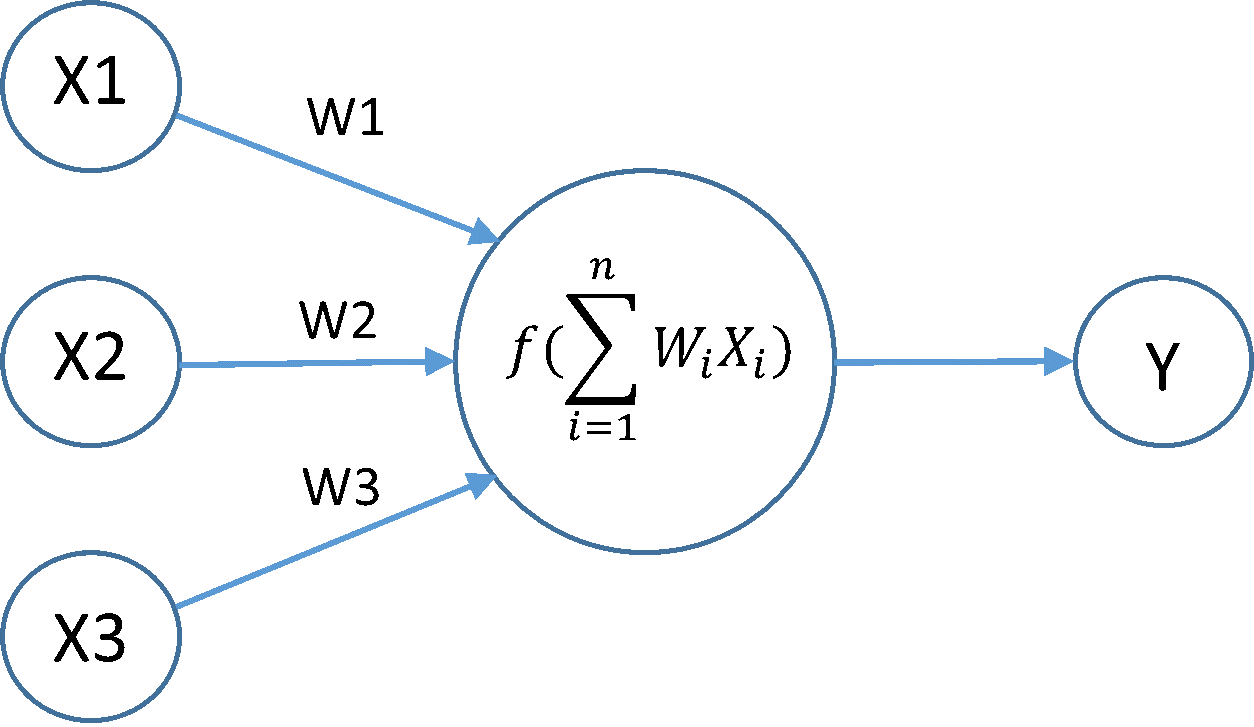
\includegraphics[width=0.4\textwidth]{neuron.png}
\caption{Neuron. From \emph{Applying Unsupervised Machine Learning to Sequence Labeling}, by Jacob, 2019. \url{https://medium.com/mosaix/deep-text-representation-for-sequence-labeling-2f2e605ed9d}. Copyright n.d. by n.d.}
\end{figure}

Many NLP applications using neural networks feed in word tokens that is transformed based on its context words, resulting in an updated version of the word embedding (Smith, 2019). Embeddings are fed as parameters or weights into a neural network which \emph{optimizes} them to best fit the text by minimizing a continuous loss function using gradient-descent based algorithms. Every neural network representation consists of three components (Ruder, 2016):

1. \textbf{Embedding Layer}: this layer creates word embeddings by multiplying an index vector with a word vector matrix. 

2. \textbf{Intermediate Layer(s)}: multiple layers are used to create a fully-connected layer that applies a non-linearity function (like hyperbolic tangent or sigmoid) to the concatenation of word embeddings. 

3. \textbf{Softmax Layer}: the last layer normalizes the word embedding matrix to produce a probability distribution over words in the vocabulary. Specifically, the softmax layer calculates the probability of word vector $w_t$ as follows: 
$$
P \Big(w_t \; | \; w_{t-1}, ..., w_{t-n+1} \Big) = \frac {\exp{ \Big(h^T \cdot v_{w_t}' \Big) }} {\sum_{w_i \in V} \exp{ \Big(h^T \cdot v_{w_i}' \Big) }}
$$
where $V = $ vocabulary of a corpus, $h = $ output vector of the hidden layer, and $v_w' = $ the output embedding of word $w$. 

\subsubsection{Solution to Curse of Dimensionality: Neural Model and Continuous Vector Representations}

The $n$-gram model seeks to remedy the \emph{curse of dimensionality} by combining short overlapping word sequences seen in the training set. 

However, Bengio et al. (2003) developed a neural probabilistic language model to learn a distributed representation for words to allow the model to generalize to unseen data. The neural model does two tasks simultaneously; (1) it learns a distributed representation for each word, and also (2) it learns the probability distribution of word sequences \emph{as a function of} the distributed representations. The model generalizes to unseen data successfully because unseen word sequences get a high probability if containing words that are similar to words that were already seen.  

Advantageously, this model can capture longer contexts better than the $n$-gram, which is limited to short contexts. As a result of continuous word vector representations, the learned probability function's parameters increase only linearly instead of exponentially, with the vocabulary size, and linearly, with vector dimension, thus resolving the curse of dimensionality (Bengio et al., 2003). 

\subsection{Bidirectional Language Model}

\subsubsection{Forward Language Model}

A general language model predicts a next word given its context words, $P(\textit{Word} \: | \: \textit{Context})$. 

However a forward language model takes this context to be previous words. Peters et al. (2018) formalizes this as:  given a sequence of $N$ tokens $(t_1, t_2, ..., t_N)$, a forward language model calculates the probability of the tokenized sentence assuming the probability of a word token $t_k$ is conditional on its history tokens, $(t_1, ..., t_{k-1})$:
$$
P \Big(t_1, t_2, ..., t_N \Big) = \prod_{k=1}^N P \Big(t_k \; | \; t_1, t_2, ..., t_{k-1} \Big)
$$

\subsubsection{Backward Language Model}

A backward language model is similar to a forward model excepts it predicts the current token $t_k$ conditional on future context tokens:
$$
P \Big(t_1, t_2, ..., t_N \Big) = \prod_{k=1}^N P \Big(t_k \; | \; t_{k+1}, t_{k+2}, ..., t_N \Big)
$$

\subsubsection{Combining Forward and Backward}

A bidirectional language model combines the forward and backward language models and uses maximum likelihood estimation to \emph{jointly} maximize the log likelihood of the forward and backward directions: 
$$
\sum_{k=1}^N \Big( \text{log} \Big( P \Big(t_k \; | \; t_1,...,t_{k-1}; \; \overrightarrow{\theta} \Big) + \text{log} \Big( P \Big(t_k \; | \; t_{k+1}, t_{k+2}, ..., t_N; \; \overrightarrow{\theta} \Big) \Big)
$$
where $\overrightarrow{\theta}$ represents additional parameters (Peters et al., 2018). 


\begin{figure}[h]
\centering
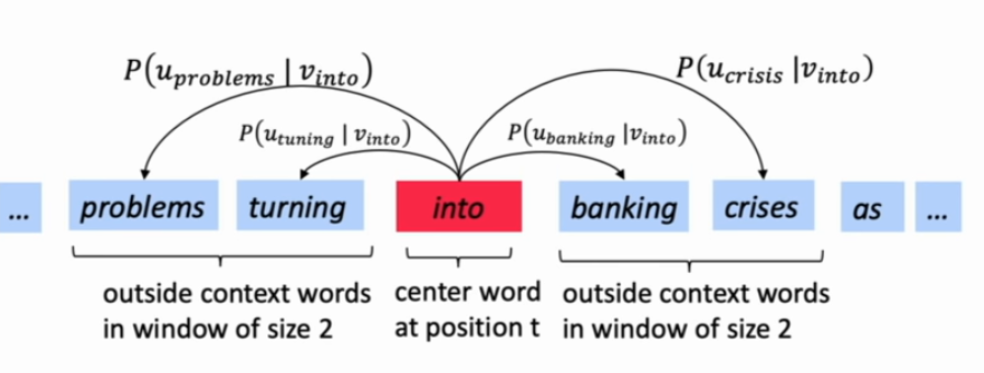
\includegraphics[width=0.6\textwidth]{bidirectional_languagemodel_banking.png}
\caption{Example Bidirectional Language Model. From \emph{Word2Vec Overview With Vectors}, by CS224n: Natural Language Processing with Deep Learning (Stanford), 2018. \url{https://sangminwoo.github.io/2019-08-28-cs224n-lec1/}. Copyright n.d. by n.d.}
\end{figure}

Akbik et al. (2018) use the hidden states of a bidirectional recurrent neural network to create contextualized word representations. 

For example, consider the sentences ``Mary accessed the bank account" and ``The swan waded to the bank of the river." In the first sentence, a unidirectional contextual model would represent the target word ``bank" based on `I accessed the' but not `account,' thus failing to capture the polysemy of `bank.' But a bidirectional language model represents ``bank" using both previous and next context to ameliorate this problem.
